\documentclass[a4paper]{article}

%% Language and font encodings
\usepackage[english]{babel}
\usepackage[utf8x]{inputenc}
\usepackage[T1]{fontenc}
\usepackage{helvet}
%\usepackage[numbers]{natbib}
\usepackage[round]{natbib}
%% For citations with atuhor et al year, usehttps://www.overleaf.com/16365895fcrtzrvgdsvp
%% \usepackage[round]{natbib}
%% \bibliographystyle{abbrv} (optional)
%% \citealt{adams1995hitchhiker}
\usepackage{upgreek} %%% This enables non-italic greek letters.
%% The lowercase letters are named \upalpha, \upbeta, ... and so, and upercase are named \Upalpha, \Upbeta, ...
%% line thickness
\usepackage{soul} %% Highlight package
\usepackage{lineno} %% Add line numbers to the document

%% Sets page size and margins
\usepackage[a4paper,top=3cm,bottom=2cm,left=3cm,right=3cm,marginparwidth=1.75cm]{geometry}
\setlength{\arrayrulewidth}{0.5mm}
\setlength{\tabcolsep}{4pt}

\renewcommand{\arraystretch}{1.3}
\newcommand{\beq}{\begin{equation}}
\newcommand{\eeq}{\end{equation}}

%% Useful packages

\usepackage{amsmath}
\usepackage{graphicx}
\usepackage[colorinlistoftodos]{todonotes}
\usepackage[colorlinks=true, allcolors=blue]{hyperref}
\usepackage{array}
\usepackage{float}
\usepackage{appendix} 
\usepackage{multirow}
\usepackage[symbol]{footmisc}
\usepackage{setspace}
\usepackage{authblk} %%% Support for footnote style author/affiliation.
\usepackage{ctable}
\renewcommand{\thefootnote}{\fnsymbol{footnote}}
\renewcommand\Affilfont{\itshape\small}
\usepackage{comment}
\usepackage{subfig}  
\usepackage{subcaption}
\usepackage{indentfirst}
\usepackage{siunitx}
\usepackage{amssymb,stmaryrd}
\usepackage{bbold}
\usepackage{enumerate}
\usepackage{enumitem}
\bibliographystyle{dinat}
\usepackage{amsthm}
%%% Packages for theorems and definitions, etc

\newtheorem{corollary}{Corollary}[section]
\newtheorem{lemma}{Lemma}[section]
\theoremstyle{definition}
\newtheorem{definition}{Definition}[section]
\newtheorem{theorem}{Theorem}

\title{SLH Formalism}
\author[1]{Antonio Cobarrubia}
\affil[1]{Department of Physics, San Diego State University, San Diego, CA 92182}

\date{}

\begin{document}

\maketitle

\doublespacing
\section{Introduction}
Here is an explanation of the composition rules of SLH and a simple example to go alongside with it. I still need to learn how to derive each SLH operation (in-progress), but here is a first look on what SLH formalism can do and how someone can apply it to basic circuits. The SLH triple for each individual component can be found through other methods, which we can use other methods/material to build the scattering matrix, coupling operator and hamiltonian. From there SLH can be applied. 
\section{Quantum Input-Output Theory}

\section*{Hamiltonian Description}
The Hamiltonian description begins with asypmtotic field descriptions of input/output fields with localized systems. The derivation of quantum input-output theory is based on Combes SLH tutorial (\citealt{Combes_2017}). This is described as the following
\begin{align*}
H_{\text{tot}} = H_{\text{sys}} + H_{\text{field}} + H_{\text{inter}} 
\end{align*}
where $H_{\text{sys}}$ is the Hamiltonian of the system, $H_{\text{field}} $ is the Hamiltonian of the bosonic field in a vacuum, and $H_{\text{inter}} $ is the Hamiltonian of interaction between the system and field (\citealp{Gardiner_2004}). For the rest of these notes, we'll assume $\hbar = 1$ unless specified. For input/output theory, the field hamiltonian in lab frame is 
$$
H_{\text{field}} = \int_0^\infty d\omega \omega b^\dagger(\omega) b(\omega)
$$
where b($\omega$) are bosonic annihiliation operators in optical-frequency space  and statisfies communtation relation [b($\omega$), $b^\dagger$($\omega$)] = $\delta(\omega - \omega')$. The interaction term takes a general form 
$$
H_{\text{inter}} = i \int_0^\infty d\omega \kappa(\omega)[b(\omega)-b^\dagger(\omega)][c-c^\dagger]
$$
where $\kappa(\omega)$ is the coupling strength and c is coupling operator. For a system and bath are weakly coupled, and utilizing rotation wave approximation (RWA) and Markov approxiamtion ($\kappa \sim \sqrt{\frac{\gamma}{2\pi}}$), the interaction term can approximated as 
\begin{align*}
    H_{\text{inter}}(t) \approx i \sqrt{\frac{\gamma}{2\pi}} \int_{-\infty}^\infty d\omega [cb^\dagger(\omega) - c^\dagger b(\omega)]
\end{align*}

The quantum Langevin equation for the evolution of an arbitrary system operator A arrives at a known input-output equation in the Heisenberg picture: 
\begin{align}
\label{eq:langevin}
    \Dot{\tilde{A}}(t) \approx -i[\tilde{A}(t), H_{\text{sys}}]-([\tilde{A}(t), c^\dagger(t)](\frac{\gamma}{2}c(t)+\sqrt{\gamma}\tilde{b}(t)) - (\frac{\gamma}{2}c^\dagger(t)+\sqrt{\gamma}\tilde{b}^\dagger(t)) [\tilde{A}(t), c(t)])
\end{align}
where $\tilde{A}(t) = A(t) \otimes \mathbb{1}_{\text{field}}$, and $\tilde{b}$(t) is the input/output field mode operator. This also known a lindblad master equation in quantum optics. The definition of an input field operator $b_{\text{in}}$(t) and output field operator $b_{\text{out}}$(t) is 
\begin{align}
    b_{\text{in}}(t) & = \frac{1}{\sqrt{2\pi}} \int d\omega b_{t = 0}(\omega)e^{-i\omega t} \\
    b_{\text{out}}(t) & = \frac{1}{\sqrt{2\pi}} \int d\omega e^{-i\omega (t-t_1)} b_{t_1}(t) 
\end{align}
 where $t_1 > t$ and $ b_{t_1}(t)$ is the value of an evolved $ b_{\text{in}}(t)$ (\cite{Gardiner_2004}). Two separate equations can be made from eq. \ref{eq:langevin} by replacing $\tilde{b}$(t) with input or output field operator .
 We can therefore define the interaction Hamiltonian  as 
 \begin{align}
     \label{eq:interaction_ham}
     H_{\text{inter}} = \textbf{L}b^\dagger_{\text{in}}-\textbf{L}^\dagger b(\omega)
 \end{align}
  where $\textbf{L}$ = i$\sqrt{\gamma}$c is the coupling/lindblad operator. This form will be modified later when discussing the unitary propagator in the perspective of Hudson and Parthasarathy solutions of quantum stochastic differential equations. Here is the basic understanding on how one will obtain the true SLH Hamiltonian formalism. 
 \begin{align}
    b_{\text{out}}(t) =  b_{\text{in}}(t) + \textbf{L}
 \end{align}
This relation can be modified by Hudson and Parthasarathy (\citealt{Gough_2008, Hudson1984}) solution to quantum stochastic differential equation (QSDE) with scattered bosonic fields: 
 \begin{align}
 \label{eq:input_outtput_relation}
     b_{\text{out}}(t) = \textbf{S} b_{\text{in}}(t) + \textbf{L}
 \end{align}
 where S is the scattering matrix with unitary conditions: $\textbf{S}\textbf{S}^\dagger = \textbf{S}^\dagger \textbf{S} = \mathbb{1}$. 
\section*{Quantum Stochasitic Differentiation}
Proper integration of input and output fields are entirely stochastic by nature. Here lets define more the stochastic transformations of classical input-output theory. The stochastic bosonic field operators is defined as 
\begin{align}
    B_{\text{in}}(t) = \int_0^t ds b_{\text{in}}(s) ; & \ \ \ \ B^\dagger_{\text{in}}(t) = \int_0^t ds b^\dagger_{\text{in}}(s) \\
    dB_{\text{in}}(t) = \int_t^{t+dt} ds b_{\text{in}}(s) ; & \ \ \ \ dB^\dagger_{\text{in}}(t) = \int_t^{t+dt} ds b^\dagger_{\text{in}}(s)
\end{align}
and the differential form of the increments of $dB_{\text{in}}$(t) is
\begin{align}
    dB_{\text{in}}(t) = b_{\text{in}}(t)dt
\end{align}
For simplicity, we'll assume b(t) = $b_t$ and $dB_\text{in}(t)$ = $dB_\text{in}$. 
For asymptotic input fields starting initially in a vacuum state, It$\Bar{o}$ integration of QSDEs conserve commutation relations for bosonic fields [$dB_{\text{in}}$, $dB^\dagger_{\text{in}}$] = dt, but it has to obey a modified chain rule (\citealp{Combes_2017,Gardiner_2004}): 
\begin{align}
    \label{eq:ito_chain}
    d(A_tB_t) = dA_tB_t + A_tdB_t + dA_tdB_t
\end{align}
The commutation relations are also known as vacuum It$\Bar{o}$ products as shown in Table \ref{tab:ito_table}. However, QSDEs was initially derived with stratonovich integration, which retains normal calculus chain rule, to capture real noise process. This calls for a correction (It$\Bar{o}$ correction) converting between forms (\citealp{Gardiner_2004}).  

\begin{table}[H]
    \centering
    \begin{tabular}{l|l l l l}

       x  & $dB_t$ & $d\Lambda_t$ & $dB^\dagger_t$ & dt\\
     \hline 
        $dB_t$ & 0 & dB & dt & 0\\
      $d\Lambda_t$ & 0 & $d\Lambda_t$ & $dB_t^\dagger$ & 0 \\
     $dB^\dagger_t$ & 0 & 0 & 0 & 0 \\
     dt & 0 & 0 & 0 & 0
    \end{tabular}
    \caption{It$\Bar{o}$ Table for vacuum field inputs.}
    \label{tab:ito_table}
\end{table}
For SLH, It$\Bar{o}$ integration provides a powerful tool to simplify equations. This table was taken from (\cite{Combes_2017}).

\section*{Unitary Propagator}
The derivation of many SLH connections depends on the evolution of a unitary propagator. SLH formalism was derived at an initial time $t_0 = 0$, the unitrary operator U(t$t_0$ = 0) is U(t). In principle, the propagator is defined as
\begin{align}
\label{eq:propagator}
    U(t) & = \tau \text{exp}\{K(t)\}; \nonumber \\
    K(t) & = \int_{t_0}^t ds[-iH_{\text{sys}} + \textbf{L}b_{\text{in}}(s)-\textbf{L}^\dagger S b_{\text{in}}(s) + (\textbf{S}-\mathbb{1})b^\dagger_{\text{in}}(s)b_{\text{in}}(s)]
\end{align}
where $\tau $ is the time order. The SLH framework is built by Hudson-Parthasarathy solutions to QSDEs, which is why the total Hamiltonian is modified to include the scattering matrix and a gauge term ($ H_{\text{gauge}}(t) = (\textbf{S}-\mathbb{1})b^\dagger_{\text{in}}(t)b_{\text{in}}(t))$. In the interest to solve eq. \ref{eq:langevin}, a unitary transformation of the arbitrary system operator ($\tilde{A}$(t) = $U(t)\tilde{A}(0)U^\dagger(t)$) is a common operation to solve, which expresses the need to known stochastic description of the differential propagator with respect to time. Here is a following proof of a QSDE of the time evolution unitary operator
\begin{align}
    \frac{dU_t}{dt} & = \tau \frac{d}{dt}(\text{exp}\{K(t)\}) \nonumber \\
    \frac{dU_t}{dt} & = \frac{dK_t}{dt} \tau \text{exp}\{K(t)\} = \frac{dK_t}{dt}U_t \nonumber \\
     dU_t & = \frac{dK_t}{dt}U_t dt = \frac{dK_t}{dt} dt U_t \nonumber \\
     dU_t & =  \Bigg( \frac{dK_t}{dt} dt \Bigg) U_t
\end{align}
where $\frac{dK_t}{dt} = -(iH_{\text{sys}} + \frac{1}{2}\textbf{L}^\dagger$\textbf{L}) + $ \textbf{L}b_{\text{in}}(t)-\textbf{L}^\dagger \textbf{S} 
b_{\text{in}}(t) + (\textbf{S}-\mathbb{1})b^\dagger_{\text{in}}(t)b_{\text{in}}(t)$, and
-$\frac{1}{2}\textbf{L}^\dagger \textbf{L}$ is the It$\Bar{o}$ correction between Stratonovich integration to It$\Bar{o}$ integration. Thus, $\frac{dK_t}{dt} dt$  known as differential germ ($dG(t) = dG_t$) (\cite{Fagnola_2019}) is defined as
\begin{align}
    dG_t & = -(iH_{\text{sys}} + \frac{1}{2}\textbf{L}^\dagger \textbf{L})dt + \textbf{L}b_{\text{in}}(t)dt-\textbf{L}^\dagger \textbf{S} b_{\text{in}}(t)dt + (\textbf{S}-\mathbb{1})b^\dagger_{\text{in}}(t)b_{\text{in}}(t) dt \nonumber \\
    dG_t & = -(iH_{\text{sys}} + \frac{1}{2}\textbf{L}^\dagger \textbf{L})dt + \textbf{L} dB^\dagger_\text{in} - \textbf{L}^\dagger \textbf{S} dB_\text{in} + (\textbf{S}-\mathbb{1})d\Lambda_t \label{eq:differential_germ}
\end{align}
where $\Lambda(t) = \int_0^t ds b^\dagger_{\text{in}}(s)b_{\text{in}}(s)$, and $d\Lambda(t) = d\Lambda_t = b^\dagger_{\text{in}}(t)b_{\text{in}}(t) dt$. The operator, $\Lambda(t)$, is the measurement of the number of field photons also known as the gauge process. Based on this, the It$\Bar{o}$ form of the unitary propagator is 
\begin{align}
\label{eq:Ito_unitary_sol}
    dU_t & =  dG_t U_t \nonumber \\
    dU(t)& =  [-(iH_{\text{sys}}(t) + \frac{1}{2}\textbf{L}^\dagger \textbf{L})dt + \textbf{L} dB^\dagger_\text{in}(t) - L^\dagger \textbf{S}dB_\text{in}(t) + (\textbf{S}-\mathbb{1})d\Lambda(t)] U(t)
\end{align}
This QSDE is also known as the Hudson-Parthasarthy equation (\cite{Fagnola_2019,Gough_2008, Hudson1984}). The formal solution to eq. \ref{eq:Ito_unitary_sol} is given by
\begin{align}
\label{eq:propagator_formal}
    U(t) & = \tau \text{exp}\{\int_{t_0}^t dG(s)\} \nonumber \\
    U(t) & = \tau \text{exp}\{\int_{t_0}^t ds[-(iH_{\text{sys}}(s) + \frac{1}{2}\textbf{L}^\dagger \textbf{L})dt + \textbf{L} dB^\dagger_\text{in}(s) - \textbf{L}^\dagger SdB_\text{in}(s) + (\textbf{S}-\mathbb{1})d\Lambda(s)] \}
\end{align}
where the modified K(t) is the integral in the exponential of eq. \ref{eq:propagator_formal}.
\begin{lemma}
The unitary matrix starting from initial state at $t_0$ = 0 to infinitesimal increment of time, t = dt, is given as U(dt,0) = $\mathbb{1}$ + dU(0).
\end{lemma}
\begin{proof}
For small increments of time, the unitary matrix won't have enough time to evolve at infinitestimal increments of time. The unitary matrix will won't have enough time to drastically evovle from its original state. Thus, a taylor expansion to the first order (O(d$t^2) \approx$ 0) of eq. \ref{eq:propagator_formal} is given by
\begin{align}
    U(dt) & \approx \mathbb{1} +  \frac{dK(0)}{dt}U(0)dt \nonumber \\
     U(dt) & \approx  \mathbb{1} + [-(iH_{\text{sys}}(0) + \frac{1}{2}\textbf{L}^\dagger \textbf{L})dt +  \textbf{L}b_{\text{in}}(0)dt-\textbf{L}^\dagger \textbf{S} b_{\text{in}}(0)dt + (\textbf{S}-\mathbb{1})b^\dagger_{\text{in}}(0)b_{\text{in}}(0)dt]U(0) \nonumber \\
     U(dt) & \approx \mathbb{1} + [-(iH_{\text{sys}}(0) + \frac{1}{2}\textbf{L}^\dagger \textbf{L})dt + \textbf{L} dB^\dagger_\text{in}(0) - \textbf{L}^\dagger \textbf{S}dB_\text{in}(0) + (\textbf{S}-\mathbb{1})d\Lambda(0)] U(0) \nonumber \\
     U(dt) & \approx \mathbb{1} + dU(0)
\end{align}

\end{proof}


\section*{Linear QSDE and Model Matrix}
In this section, we can develop SLH theory in terms of linear quantum systems with negligible time delays, or systems that converges to a Model (\citealp{Combes_2017,Hudson1984, Nurdin_2010}). The stochastic differential equations derived by Hudson-Parthasarthy is given by two stochastic equations: differential germ and stochastic input-output relation (\citealp{Gough_2008}).  
Incremental changes of output field $dB_{\text{out}}$ allows us to measure the final state of a bosonic field after fed through quantum optical components. The modified QSDE-proved by Hudson and Parthasarthy  for arbitrary output operators (\citealp{Hudson1984})-to eq. \ref{eq:input_outtput_relation},  is as follows
\begin{align}
    \frac{db_{\text{out}}(t)}{dt} & = \textbf{S} b_{\text{in}}(t) + \textbf{L} \nonumber \\
    db_{\text{out}}(t) & = \textbf{S} b_{\text{in}}(t) dt + \textbf{L} dt \nonumber \\ 
    db_{\text{out}}(t) & = \textbf{S} dB_{\text{in}}(t) + \textbf{L} dt \label{eq:input_outtput_relation_QSDE}
\end{align}
For linear systems, one derive the equations of motion for internal degrees of freedom based on eq. \ref{eq:differential_germ} and eq. \ref{eq:input_outtput_relation_QSDE}. The linear relationship between the two QSDEs is as follows:
\begin{align*}
     dG(t) & = -(iH_{\text{sys}} + \frac{1}{2}\textbf{L}^\dagger \textbf{L}) dt  - \textbf{L}^\dagger \textbf{S} dB_\text{in} + \textbf{L} dB^\dagger_\text{in} + (\textbf{S}-\mathbb{1})d\Lambda_t \\
    db_{\text{out}} & = \textbf{L} dt +  \textbf{S} dB_{\text{in}} 
\end{align*}
Here we can represent the SLH triple through linear matrices described by 
\begin{align}
   \begin{bmatrix}
dG_t \\
db_{\text{out}}
\end{bmatrix} & = 
\begin{pmatrix}
-(iH_{\text{sys}} + \frac{1}{2}\textbf{L}^\dagger \textbf{L}) & - \textbf{L}^\dagger \textbf{S} \\
\textbf{L} & \textbf{S}
\end{pmatrix} 
\begin{bmatrix}
dt \\
dB_\text{in} 
\end{bmatrix}+ 
\begin{pmatrix}
\textbf{L} & (\textbf{S}-\mathbb{1}) \\
0 & 0
\end{pmatrix} 
\begin{bmatrix}
dB^\dagger_\text{in} \\
d\Lambda_t
\end{bmatrix}
\label{eq:model_matrix_eq}
\end{align}
The linear matrices describes the SLH triple:
\begin{align}
    \textbf{V} = \begin{pmatrix}
-(iH_{\text{sys}} + \frac{1}{2}\textbf{L}^\dagger \textbf{L}) & - \textbf{L}^\dagger \textbf{S} \\
\textbf{L} & \textbf{S}
\end{pmatrix}; &  \textbf{M} = \begin{pmatrix}
\textbf{L} & (\textbf{S}-\mathbb{1}) \\
0 & 0
\end{pmatrix} \label{eq:model_matrix_formal}
\end{align}
The matrix \textbf{V} is known as a model matrix (\citealp{Gough_2008, Nurdin_2010}). We'll refer to this as the normal form of the SLH triple in terms model matrix representation. This model matrix will be useful to derive important SLH connections. In particular, this will be useful to prove the concatenation product.

\begin{definition}
\textbf{(Gough, Definition 9). (\citealp{Gough_2008})}. For a Hamiltonian $H_N$ for a quantum network N with a model matrix \textbf{V} (eq. \ref{eq:model_matrix_formal}) and m amount of edges e = (r, s) (connection of an input channel r to an output channel s) is an operator of the network Hilbert's space if all Sobolev-Fock vectors $\Phi$ in the network's domain satisfy the boundary conditions 
\begin{align}
    b_{\text{out,s}}(T^-_s) \Phi & = \sum_r V_{sr} b_{\text{in,r}}(T^+_r) \Phi \label{eq:model_input/output_relation} \\
    -iH_N \Phi & = \sum_r V_{0r} b_{\text{in,r}}(T^+_r) \Phi - iH_0 \Phi \label{eq:model_hamiltonian} \\
    b_{e}(T^+_r) = b_{\text{in,r}}(T^+_r) =  \lim_{t\to T^+_r} b_{r}(t); \ & \ b_{e}(T^-_s) = b_{\text{out,s}}(T^-_s) = \lim_{t\to T^-_s} b_{s}(t) \nonumber \\
        & \nonumber \\
    V_{00} =  -\sum_{s\in P_{\text{in}}(N)} (iH_{\text{sys}} + \frac{1}{2}L_s^\dagger L_s); \ & \ V_{0r} = - \sum_{s\in P_{\text{out}}(N)} L_s^\dagger S_{sr} \nonumber \\
    V_{s0} = L_s; \ & \ V_{sr} = S_{sr} \nonumber
\end{align}
where $r \in \{0\} \bigcup P_{\text{in}}$(N), $s \in \{0\} \bigcup P_{\text{out}}$(N), r is the input channel, s is the output channel, $ P_{\text{in}}$(N) is the set of input channels $\{r_1, \dots, r_m\}$ $ P_{\text{out}}$(N) is the set of input channels $\{s_1, \dots, s_m\}$, $\tau = T_s - T_r$ be the time delay of a bosonic field to travel between r and s, and $H_0 = \sum_j \int_{T_r}^{T_s} b^\dagger_{e,j}(t)i\frac{\delta}{\delta t}b_{e,j}(t)dt$. 

\end{definition}

\section{Basic Algebraic Rules of SLH}
The SLH composition rules are algebraic descriptions of combining components in various manners, under asymptotic free fields approximation. These rules will give us insight on how to evaluate (optical) circuit components.





\section*{Series Product}
\begin{enumerate}[label=(\roman*)]
\item
\textbf{Composition Rule}: 

\begin{figure}[H]
\centering
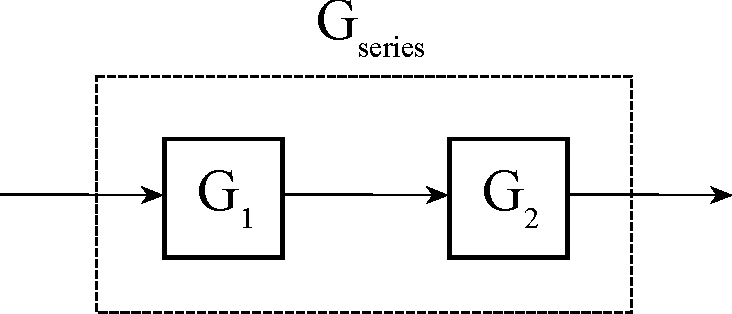
\includegraphics[width = 7.5 cm]{Series_Product.pdf}
\caption{Series of component $G_1$ output is cascaded into the input of $G_2$.
}
\label{fig:series}
\end{figure}  


\theoremstyle{definition}
\begin{definition}{Series Product.}
For two components connected in series, where the output of $G_1$ = ($S_1,L_1,H_1$) is sent into the input of $G_2 = (S_2, L_2, H_2)$ is called a \textit{series product} ($\triangleleft$), or \textit{cascade rule}, as seen in Figure \ref{fig:series}. The ith number of inputs/outputs in $G_1$ have to be the same number of jth input/output of $G_2$. This connection is directional, where the series product is not equivalent if the output of 2 goes into the input of 1 ($ G_2 \triangleleft G_1 \ne G_1 \triangleleft G_2$ ).


\begin{align*}
    G_{\text{series}} = & \ G_2 \triangleleft G_1 \\
    G_{\text{series}} = & \ (\textbf{S}_2,\textbf{L}_2,H_2) \triangleleft (\textbf{S}_1,\textbf{L}_1,H_1)
\end{align*}
\begin{align}
    G_{\text{series}} = & \ \Bigg( \textbf{S}_2\textbf{S}_1,\textbf{L}_2+\textbf{S}_2\textbf{L}_1,H_1 + H_2 + \frac{1}{2i}(\textbf{L}_2^\dagger \textbf{S}_2\textbf{L}_1 - \textbf{L}_1^\dagger \textbf{S}_2^\dagger \textbf{L}_2) \Bigg) 
    \label{eq:series}
\end{align}
\end{definition}
\item
\begin{proof}
Let use assume the SLH triple of $G_1$ and $G_2$ are coupled from the out-port of $G_1$ with the in-port of $G_2$ (\cite{Kockum_2012}). Assume there is no time delay between the two components, however, the field state measured by $G_1$ is the input field state of $G_2$. For small increments of time, the evolution of the total propagation of the unitary operator is given by dt for $G_1$ then by $G_2$ then another increment of time of $G_1$, and henceforth. Using the well known property of unitary propagator ($U(t_c,t_a) = U(t_c,t_b)U(t_b,t_a)$), the first cycle (from 0 to $t_1$) of the total unitary matrix is given as 
\begin{align}
    U_{\text{tot}}(t_1,0) & = U_2(dt)U_2(dt) = (\mathbb{1}+dU_2(0))(\mathbb{1}+dU_1(0)) \nonumber \\
    U_{\text{tot}}(t_1,0) & = \mathbb{1}\mathbb{1} + dU_2(0)\mathbb{1} + \mathbb{1}dU_1(0) + dU_2(0)dU_1(0)  \nonumber \\
    U_{\text{tot}}(t_1,0) & = \mathbb{1} +  dU_2(0) + dU_1(0) + dU_2(0)dU_1(0) \ + \nonumber \\ 
    U_{\text{tot}}(t_1,0) & = \mathbb{1} + [-(iH_{2} +  \frac{1}{2}\textbf{L}_2^\dagger \textbf{L}_2)dt + L_2 dB^\dagger_0 - \textbf{L}_2^\dagger \textbf{S}_2dB_0 + (\textbf{S}_2-\mathbb{1} d\Lambda(0)] U(0) \ + \nonumber \\
     & \ [-(iH_{1} + \frac{1}{2}\textbf{L}_1^\dagger \textbf{L}_1)dt + \textbf{L}_1 dB^\dagger_0 - \textbf{L}_1^\dagger \textbf{S}_1 dB_0 + (\textbf{S}_1-\mathbb{1})d\Lambda_0] U(0) \ + \nonumber \\ 
     & \ dU_2(0)dU_1(0) \label{eq:seriers_proof_1}
\end{align}
where $dB_{\text{in}}(0) = dB_0$, $d\lambda(0) = d\Lambda_0$,$H_1(0) = H_1$, and $H_2(0) = H_2$. Before we proceed with the last term, we can easily see from Table \ref{tab:ito_table} that the only contributing terms from only $dU_2(0)dU_1(0)$ are when their It$\Bar{o}$ product isn't zero. These products are defined as 
\begin{align}
    (-\textbf{L}_2^\dagger \textbf{S}_2)(\textbf{L}_1) dB_0dB_0^\dagger & = (-\textbf{L}_2^\dagger \textbf{S}_2\textbf{L}_1) dt \label{eq:ito_dbdbdag} \\
    (-\textbf{L}_2^\dagger \textbf{S}_2)(\textbf{S}_1-\textbf{$\mathbb{1}$}) dB_0d\Lambda_0 & = (\textbf{L}_2^\dagger \textbf{S}_2-\textbf{L}_2^\dagger \textbf{S}_2\textbf{S}_1) dB_0 \label{eq:ito_dbdl} \\
    (\textbf{S}_2-\textbf{$\mathbb{1}$})(\textbf{L}_1)d\Lambda_0 dB_0^\dagger  & = (\textbf{S}_2\textbf{L}_1-\textbf{L}_1) dB^\dagger_0 \label{ito_dbdagdl} \\
    (\textbf{S}_2-\textbf{$\mathbb{1}$})(\textbf{S}_1-\textbf{$\mathbb{1}$})d\Lambda_0d\Lambda_0 & = (\textbf{S}_2\textbf{S}_1 - \textbf{S}_2 - \textbf{S}_1 + \textbf{$\mathbb{1}$}) d\Lambda_0 \label{eq:ito_dldl}
\end{align}
Now, we'll plug the results of eq. \ref{eq:ito_dbdbdag}-\ref{eq:ito_dldl} into eq. \ref{eq:seriers_proof_1} the result of $dU_2(0)dU_1(0)$, and group terms based on there differential product:
\begin{align}
    U_{\text{tot}}(t_1,0) & = [-i(H_1+H_2) - \frac{1}{2}(\textbf{L}_1^\dagger \textbf{L}_1 + \textbf{L}_2^\dagger \textbf{L}_2) - \textbf{L}_2^\dagger \textbf{S}_2\textbf{L}_1] dt \ +  \nonumber \\
    & \ [\textbf{L}_1 + \textbf{L}_2 + (\textbf{L}_2\textbf{S}_2-\textbf{L}_2)]dB_0^\dagger \ + \nonumber \\
    & [-\textbf{L}_1^\dagger \textbf{S}_1 - \textbf{L}_2^\dagger \textbf{S}_2 + (\textbf{L}_2^\dagger \textbf{S}_2-\textbf{L}_2^\dagger \textbf{S}_2\textbf{S}_1)] dB_0 \ + \nonumber \\
    & [(\textbf{S}_1-\mathbb{1}) + (\textbf{S}_2-\mathbb{1}) + (\textbf{S}_2\textbf{S}_1 - \textbf{S}_2 - \textbf{S}_1 + \mathbb{1}) ] d\Lambda_0 \nonumber \\
    U_{\text{tot}}(t_1,0) & = [-i(H_1+H_2 + \frac{1}{i}\textbf{L}_2^\dagger \textbf{S}_2\textbf{L}_1) - \frac{1}{2}(\textbf{L}_1^\dagger \textbf{L}_1 + \textbf{L}_2^\dagger \textbf{L}_2)] dt \ +  \nonumber \\
    & \ [\textbf{L}_2 + \textbf{S}_2\textbf{L}_1] dB_0^\dagger - [\textbf{L}_1^\dagger \textbf{S}_1 + \textbf{L}_2^\dagger \textbf{S}_2\textbf{S}_1)] dB_0 +  [\textbf{S}_2\textbf{S}_1  - \mathbb{1} ] d\Lambda_0  
\end{align}
First we can see that only the imaginary part of $\textbf{L}_2^\dagger \textbf{S}_2\textbf{L}_1$ will contribute, thus we can use a known property of imaginary numbers (z = a + ib) where $\mathbb{Im}\{z\}$= $\frac{z-z*}{2}$. The adjoint of $\textbf{L}_2^\dagger \textbf{S}_2\textbf{L}_1$ has an equivalent statement, where $\mathbb{Im}\{\textbf{L}_2^\dagger \textbf{S}_2\textbf{L}_1\} = \frac{1}{2}(\textbf{L}_2^\dagger \textbf{S}_2\textbf{L}_1 - \textbf{L}_1^\dagger \textbf{S}_2^\dagger \textbf{L}_2)$. The It$\Bar{o}$ correction terms ($\frac{1}{2}(\textbf{L}_1^\dagger \textbf{L}_1 + \textbf{L}_2^\dagger \textbf{L}_2)$) is the total It$\Bar{o}$ correction of the series connection. For the $dB_0$ components we can factor a $\textbf{S}_2\textbf{S}_1$ since the scattering matrix is unitary matrix.
\begin{align}
    U_{\text{tot}}(t_1,0) & = [-i(H_1+H_2 + \frac{1}{2i}(\textbf{L}_2^\dagger \textbf{S}_2\textbf{L}_1 - \textbf{L}_1^\dagger \textbf{S}_2^\dagger \textbf{L}_2)) - \frac{1}{2}(\textbf{L}_1^\dagger \textbf{L}_1 + \textbf{L}_2^\dagger \textbf{L}_2)] dt \ +  \nonumber \\
    & \ [\textbf{L}_2 + \textbf{S}_2\textbf{L}_1] dB_0^\dagger - (\textbf{L}_1^\dagger \textbf{S}_2^\dagger + \textbf{L}_2^\dagger) \textbf{S}_2\textbf{S}_1)] dB_0 +  [\textbf{S}_2\textbf{S}_1  - \mathbb{1} ] d\Lambda_0  \label{eq:series_total_unitary_formal}
\end{align}

Now we can compare with the normal form of a unitary matrix, eq. (\ref{eq:propagator_formal}, under input-output theory. The equivalent SLH triple of the series connection $G_T(\textbf{S}_T,\textbf{L}_T,H_T)$ is as follows: 
\begin{align*}
    \textbf{S}_T & = \textbf{S}_2\textbf{S}_1 \\
    \textbf{L}_T & = \textbf{L}_2 + \textbf{S}_2\textbf{L}_1 \\
    H_T & = H_1+H_2 + \frac{1}{2i}(\textbf{L}_2^\dagger \textbf{S}_2\textbf{L}_1 - \textbf{L}_1^\dagger \textbf{S}_2^\dagger \textbf{L}_2)
\end{align*}
Equation \ref{eq:series} is proved.

\end{proof}

Another proof of this connection is examined by a model matrix representation of a modified  eq. \ref{eq:model_matrix_eq} and comparing the result to the normal form of the SLH model matrix V  from eq. \ref{eq:model_matrix_formal} (\citealp{Gough_2008}).
\end{enumerate}


\section*{Concatenation Product}
\begin{enumerate}[label=(\roman*)]
\item
\textbf{Composition Rule}: 
\begin{figure}[H]
\centering
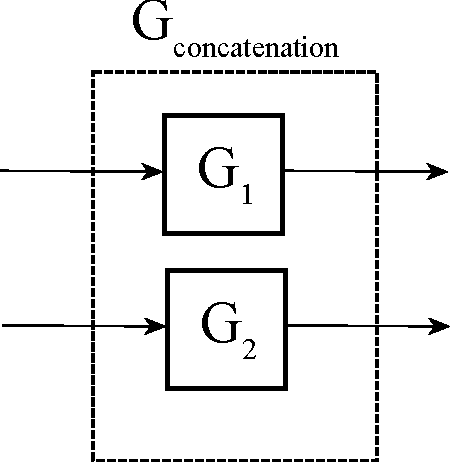
\includegraphics[width = 7.5 cm]{Concatenation_product.pdf}
\caption{A parallel connection known as a concatenation product of $G_1$ and $G_2$.
}
\label{fig:concatenation}
\end{figure}  


\theoremstyle{definition}
\begin{definition}{Concatenation Product.}
Components that are grouped in weakly coupled parallel connection is denoted as the concatenation product ($ \boxplus $) as seen in Figure \ref{fig:concatenation}. This connection is more universal, where a component direction isn't localized like the series product. The following connection is defined by



\begin{align*}
    G_{\text{concatenation}} = & \ G_1 \boxplus G_2 \\
    G_{\text{concatenation}} = & \ (\textbf{S}_1,\textbf{L}_1,H_1) \boxplus (\textbf{S}_2,\textbf{L}_2,H_2)
\end{align*}
\begin{align}
    G_{\text{concatenation}} = & \ \Bigg( \begin{pmatrix} \textbf{S}_1 & 0 \\ 0 & \textbf{S}_1\end{pmatrix},\begin{bmatrix} \textbf{L}_1 \\ \textbf{L}_2 \end{bmatrix},H_1 + H_2 \Bigg)
    \label{eq:concatenation}
\end{align}
\end{definition}
\item
\begin{proof}
Following a proof devised by Gough (\citealp{Gough_2008}), using model matrix to derive the connection. Lets define the first component as $G_1$ and $G_2$ in a parallel connection as shown in Figure \ref{fig:concatenation}. Here we'll modify our overall Hamiltonian combination of the total Hamiltonian of $G_1$ and total Hamiltonian of $G_2$:
\begin{align}
    H_T & = H^1_T + H^2_T
\end{align}
where $H^1_T$ is the total Hamiltonian of $G_1$, and $H^2_T$ is the total Hamiltonian of $G_2$. This new Hamiltonian then will redefine our unitary propagator. It is easy to see from our Hamiltonian Formulation and Unitary Propagator sections, the modified differential germ as the following:
\begin{align}
    dG^T_t & = dG^1_t + dG^2_t \nonumber \\
    dG^T_t & = -(i(H_1 + H_2) - \frac{1}{2}(\textbf{L}_1^\dagger \textbf{L}_1 + \textbf{L}_2^\dagger \textbf{L}_2))dt + \textbf{L}_1 dB^\dagger_\text{in,1} - \textbf{L}_1^\dagger \textbf{S}_1 dB_\text{in,1} + (\textbf{S}_1-\mathbb{1}) d\Lambda^1_t  \nonumber \\ 
    &  \ + \textbf{L}_2 dB^\dagger_\text{in,2} - \textbf{L}_2^\dagger \textbf{S}_2 dB_\text{in,2} + (\textbf{S}_2-\mathbb{1}) d\Lambda^2_t 
\end{align}
where $dB_\text{in,1}$ is the input field of component $G_1$, $dB_\text{in,2}$ is the input field of component $G_2$, $d\Lambda^1_t $ is the gauge process of $G_1$, and $d\Lambda^2_t $ is the gauge process of $G_2$. There will be two input-output fields associated with their respective components, which means there is two input-output QSDEs of the form eq. \ref{eq:input_outtput_relation_QSDE}: 
\begin{align*}
    db_{\text{out,1}}(t) & = \textbf{L}_1 dt + \textbf{S}_1 dB_{\text{in,1}}(t)  \\ 
    db_{\text{out,2}}(t) & = \textbf{L}_2 dt + \textbf{S}_2 dB_{\text{in,2}}(t) 
\end{align*}
Thus, the following QSDEs are define as
\begin{align}
    dG_t & = -(i(H_1 + H_2) - \frac{1}{2}(\textbf{L}_1^\dagger \textbf{L}_1 + \textbf{L}_2^\dagger \textbf{L}_2))dt + \textbf{L}_1 dB^\dagger_\text{in,1} - \textbf{L}_1^\dagger \textbf{S}_1 dB_\text{in,1} + (\textbf{S}_1-\mathbb{1}) d\Lambda^1_t  \nonumber \\ 
    &  \ + \textbf{L}_2 dB^\dagger_\text{in,2} - \textbf{L}_2^\dagger \textbf{S}_2 dB_\text{in,2} + (\textbf{S}_2-\mathbb{1}) d\Lambda^2_t \label{eq:con_group1} \\
    db_{\text{out,1}}(t) & = \textbf{L}_1 dt + \textbf{S}_1 dB_{\text{in,1}}(t)  \label{eq:con_group2} \\ 
    db_{\text{out,2}}(t) & = \textbf{L}_2 dt + \textbf{S}_2 dB_{\text{in,2}}(t) \label{eq:con_group3}
\end{align}
Equations \ref{eq:con_group1} - \ref{eq:con_group3} can make a linear combination of a modified eq. \ref{eq:model_matrix_eq}: 
\begin{align}
    \begin{bmatrix}
    dG^T_t \\
    db_{\text{out,1}}(t) \\
    db_{\text{out,2}}(t)
    \end{bmatrix} & = 
    \begin{pmatrix}
     -(i(H_1 + H_2) - \frac{1}{2}(\textbf{L}_1^\dagger \textbf{L}_1 + \textbf{L}_2^\dagger \textbf{L}_2)) & - \textbf{L}_1^\dagger \textbf{S}_1 & - \textbf{L}_2^\dagger \textbf{S}_2 \\
     \textbf{L}_1 & \textbf{S}_1 & 0 \\
     \textbf{L}_2 & 0 & \textbf{S}_2
    \end{pmatrix}
    \begin{bmatrix}
    dt \\
    dB_\text{in,1} \\
    dB_\text{in,2}
    \end{bmatrix} \ + \nonumber \\
    & \
    \begin{pmatrix}
    \textbf{L}_1 & \textbf{L}_2 & (\textbf{S}_1-\mathbb{1}) & (\textbf{S}_2-\mathbb{1}) \\
    0 & 0 & 0 & 0 \\
    0 & 0 & 0 & 0
    \end{pmatrix}
    \begin{bmatrix}
    dB^\dagger_\text{in,1} \\
    dB^\dagger_\text{in,2} \\
    d\Lambda^1_t \\
    d\Lambda^2_t
    \end{bmatrix}
\end{align}
Let's define the total scattering matrix as $\textbf{S}_T = \begin{pmatrix}
\textbf{S}_1 & 0 \\
0 & \textbf{S}_2
\end{pmatrix}$, the total Lindblad operator as 
$\textbf{L}_T = \begin{bmatrix}
\textbf{L}_1 \\
\textbf{L}_2
\end{bmatrix}$, and the total hamiltonian $H_T$ as $H_1 +H_2$ where $\frac{1}{2}(\textbf{L}_1^\dagger \textbf{L}_1 + \textbf{L}_2^\dagger \textbf{L}_2))$ is the total It$\Bar{0}$ connection. The adjoint of $\textbf{L}_T$ is $\begin{bmatrix}
\textbf{L}^\dagger_1 & \textbf{L}^\dagger_2
\end{bmatrix}$, where $-\textbf{L}_T\textbf{S}_T$ equals $\begin{bmatrix}
-\textbf{L}^\dagger_1\textbf{S}_1 & -\textbf{L}^\dagger_2 \textbf{S}_2
\end{bmatrix}$. In comparison with the normal form of the model matrix eq. \ref{eq:model_matrix_formal}, we have proved the concatenation product (eq. \ref{eq:concatenation}). 
\end{proof}

\end{enumerate}
\section*{Direct Coupling}
\begin{enumerate}[label=(\roman*)]
\item 
\textbf{Composition Rule}: 
\begin{figure}[H]
\centering
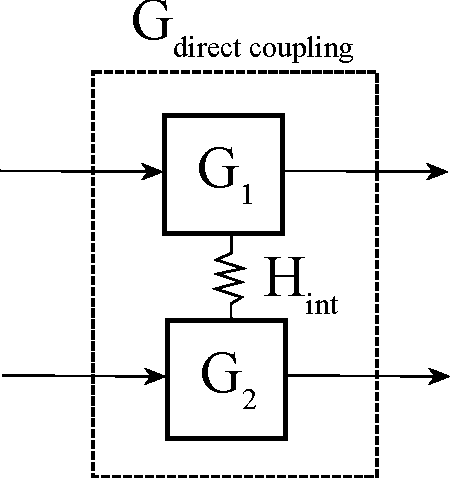
\includegraphics[width = 7.5 cm]{Direct_coupling.pdf}
\caption{Parallel connection with direct coupling of some interaction hamiltonian $H_{\text{int}}$ between $G_1$ and $G_2$. 
}
\label{fig:direct_coupling}
\end{figure}  
\begin{definition}
Direct coupling product. The direct coupling  ($\bowtie$)  of two SLH components is a special rule of a concatenation product, where there an additional interaction Hamiltonian, as shown in Figure \ref{fig:direct_coupling}. The same method of concatentaion product applies to direct coupling, but with an additional interaction Hamiltonian included of the total equivalent SLH triple. 

\begin{align*}
    G_{\text{direct coupling}} = & \ G_1 \bowtie G_2 \\
    G_{\text{direct coupling}} = & \ (\textbf{S}_1,\textbf{L}_1,H_1) \bowtie (\textbf{S}_2,\textbf{L}_2,H_2)
\end{align*}
\begin{align}
    G_{\text{direct coupling}} = & \ \Bigg( \begin{pmatrix} \textbf{S}_1 & 0 \\ 0 & \textbf{S}_1\end{pmatrix},\begin{bmatrix} \textbf{L}_1 \\ \textbf{L}_2 \end{bmatrix},H_1 + H_2 + H_{\text{int}} \Bigg)
    \label{eq:direct_coupling}
\end{align}
\end{definition}
\item
\begin{proof}
This connection is essentially a concatenation product with an added interaction term. Thus, if we follow the same exact procedure as the proof for concatenation product, but with an additional interaction Hamiltonian we'll arrive at the direct coupling connection. The differential germ is defined as $dG^T_t = dG^1_t + dG^2_t - iH_{\text{inter}}dt$. The modified QSDEs is as follows: 
\begin{align}
    \begin{bmatrix}
    dG^T_t \\
    db_{\text{out,1}}(t) \\
    db_{\text{out,2}}(t)
    \end{bmatrix} & = 
    \begin{pmatrix}
     -(i(H_1 + H_2 + H_{\text{inter}}) + \frac{1}{2}(\textbf{L}_1^\dagger \textbf{L}_1 + \textbf{L}_2^\dagger \textbf{L}_2)) & - \textbf{L}_1^\dagger \textbf{S}_1 & - \textbf{L}_2^\dagger \textbf{S}_2 \\
     \textbf{L}_1 & \textbf{S}_1 & 0 \\
     \textbf{L}_2 & 0 & \textbf{S}_2
    \end{pmatrix}
    \begin{bmatrix}
    dt \\
    dB_\text{in,1} \\
    dB_\text{in,2}
    \end{bmatrix} \ + \nonumber \\
    & \
    \begin{pmatrix}
    \textbf{L}_1 & \textbf{L}_2 & (\textbf{S}_1-\mathbb{1}) & (\textbf{S}_2-\mathbb{1}) \\
    0 & 0 & 0 & 0 \\
    0 & 0 & 0 & 0
    \end{pmatrix}
    \begin{bmatrix}
    dB^\dagger_\text{in,1} \\
    dB^\dagger_\text{in,2} \\
    d\Lambda^1_t \\
    d\Lambda^2_t
    \end{bmatrix}
\end{align}
where the modified model matrix is described as 
\begin{align}
    V_{\textbf{dc}} & =  \begin{pmatrix}
     -(i(H_1 + H_2 + H_{\text{inter}}) - \frac{1}{2}(\textbf{L}_1^\dagger \textbf{L}_1 + \textbf{L}_2^\dagger \textbf{L}_2)) & - \textbf{L}_1^\dagger \textbf{S}_1 & - \textbf{L}_2^\dagger \textbf{S}_2 \\
     \textbf{L}_1 & \textbf{S}_1 & 0 \\
     \textbf{L}_2 & 0 & \textbf{S}_2
    \end{pmatrix}
\end{align}
Adapting the equation to the normal form of the model matrix, the SLH triple is defined as the following:  $\textbf{S}_T = \begin{pmatrix}
\textbf{S}_1 & 0 \\
0 & \textbf{S}_2
\end{pmatrix}$, the total Lindblad operator as 
$\textbf{L}_T = \begin{bmatrix}
\textbf{L}_1 \\
\textbf{L}_2
\end{bmatrix}$, and the total hamiltonian $H_T$ as $H_1 + H_2 + H_{\text{inter}}$ where $\frac{1}{2}(\textbf{L}_1^\dagger \textbf{L}_1 + \textbf{L}_2^\dagger \textbf{L}_2))$ is the total It$\Bar{0}$ connection. The adjoint of $\textbf{L}_T$ is $\begin{bmatrix}
\textbf{L}^\dagger_1 & \textbf{L}^\dagger_2
\end{bmatrix}$, where $-\textbf{L}_T\textbf{S}_T$ equals $\begin{bmatrix}
-\textbf{L}^\dagger_1\textbf{S}_1 & -\textbf{L}^\dagger_2 \textbf{S}_2
\end{bmatrix}$.
\end{proof}
Note: The previous rules were derived with a vacuum source term using weak coupling approximations like the rotating wave approximation. The direct coupling rule will help construct more complicated systems using simple algebraic operations.
\end{enumerate}
\section*{Feedback Reduction}
\begin{enumerate}[label=(\roman*)]
\item
\textbf{Composition Rule}: 

\begin{figure}[H]
\centering
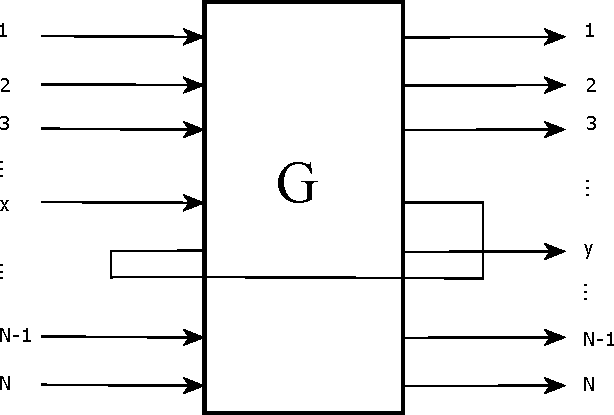
\includegraphics[width = 7.5 cm]{Feedback.pdf}
\caption{A cascaded system where the output of one port is connected to the input of another in the same component. This figure is taken from reference (\citealp{Combes_2017}).
}
\label{fig:feedback_reduction}
\end{figure}  
\begin{definition}
The feedback reduction rule is a special rule for cascaded systems, shown in Figure \ref{fig:feedback_reduction}. This rule is a derivative of the series product by splitting a component with m amount of ports into mth amount of individual components, and connecting the xth output port to the yth input port. The symbol of such rule is denoted as x $ \rightarrow \ $y. For individual components connected in a feedback reduction loop as seen in Figure \ref{fig:circuit}(a), all components are treated as an unconnected concatenation product then the reduction feedback rules apply to this unconnected form since we can build a model matrix in the form of a concatenation product. 


\begin{align*}
    G_{x \rightarrow y} = & \ \Bigg( \textbf{S}_{\text{reduction}}, \textbf{L}_{\text{reduction}}, H_{\text{reduction}} \Bigg) \\
\end{align*}
\begin{align}
\textbf{S}_{\text{reduction}} = & \ \textbf{S}_{\Bar{x}\Bar{y}} + \textbf{S}_{\Bar{x},y}(\mathbb{1}_{reduced}-S_{(x,y)})^{-1}\textbf{S}_{x,\Bar{y}} \\
\textbf{L}_{\text{reduction}} = & \ \textbf{L}_{\Bar{x}}+\textbf{S}_{\Bar{x},y}(\mathbb{1}_{reduced}-S_{(x,y)})^{-1}L_{(x)} \\
H_{\text{reduction}} = & \ H + \frac{1}{2i}(\textbf{L}^\dagger \textbf{S}_{:,y}(\mathbb{1}_{reduced}-S_{(x,y)})^{-1}L_{(x)} - L_{(x)}^\dagger (\mathbb{1}_{reduced}-S^\dagger_{(x,y)})^{-1}\textbf{S}^\dagger_{:,y}\textbf{L}) 
    \label{eq:feedback}
\end{align}
where $\textbf{S}_{\Bar{x}\Bar{y}} $ is the \textbf{S} matrix without the xth and yth row; $\textbf{S}_{\Bar{x},y}$ is the yth column of the \textbf{S} matrix without the x row (visa versa with $\textbf{S}_{x,\Bar{y}}$); $S_{(x,y)}$ is the xth and yth component of the \textbf{S} matrix; $\textbf{S}_{:,y}$ is the entire yth column of the \textbf{S} matrix; $\textbf{L}_{\Bar{x}}$ is the \textbf{L} vector without the xth row; $L_x$ is the x component of the \textbf{L} vector. The identity matrix $\mathbb{1}_{reduced}$ in the reduced SLH, has dimensions of the reduced Hilbert space.
\end{definition}
\item 
\begin{proof}
Following a proof developed by Gough (\cite{Gough_2008}), let $e_0 = (y,x)$ be a connection between two internal channels with a negligible time delay $\tau_0 \ge 0$ for an SLH triple G(\textbf{S},\textbf{L},H), Figure \ref{fig:feedback_reduction}. Propose that ($\mathbb{1}_{(m-1)X(m-1)} - V_{(x,y)}$) is invertible. For Sobolev-Fock vectors $\Phi$, the field of $x$ at $T^-_{x}$ converges to the field of $y$ at $T^+_{y}$ as $\tau_0 \rightarrow 0^+$ ($\lim_{t\to \tau_0} b_{x}(t) \Phi \rightarrow \lim_{t\to T^+_{y}} b_{y}(t)\Phi$). The boundary condition eq. \ref{eq:model_input/output_relation} can be written as 
\begin{align}
    b_{\text{out,$x$}}(T^-_{x})\Phi & = \sum_{r}V_{xr}b_{\text{in,r}}\Phi  = b_{\text{in,$y$}}(T^+_{y})\Phi \nonumber \\
    b_{\text{in,$y$}}(T^+_{y})\Phi & = V_{xy}b_{\text{in,y}}(T^+_{y})\Phi + \sum_{r'}V_{xr'}b_{\text{in,r'}}(T^+_{r'})\Phi \nonumber \\
    (\mathbb{1}_{red}-V_{xy})b_{\text{in,y}}(T^+_{y})\Phi & = \sum_{r'}V_{xr'}b_{\text{in,r'}}(T^+_{r'})\Phi \nonumber \\
     b_{\text{in,y}}(T^+_{y})\Phi & = (\mathbb{1}_{red}-V_{(x,y)})^{-1}\sum_{r'}V_{xr'}b_{\text{in,r'}}(T^+_{r'})\Phi
\end{align}
where $\mathbb{1}_{red}$ is the reduced identity matrix ($\mathbb{1}_{(m-1)X(m-1)}$), r' $\in \{0\} \bigcup \frac{P_{\text{in}}(G)}{\{y\}}$, $\frac{P_{\text{in}}(G)}{\{y\}}$ is the set of input channels excluding the yth channel, and, for future references in the proof,  s' $\in \{0\} \bigcup \frac{P_{\text{out}}(G)}{\{x\}}$ with $\frac{P_{\text{out}}(G)}{\{x\}}$ being the set of output channels excluding the xth channel.  \\
For the boundary condition using eq. \ref{eq:model_input/output_relation} for s' is given as 
\begin{align}
      \sum_{s'}b_{\text{out,s'}}(T^-_{s'})\Phi & = \sum_{s'}\sum_{r}V_{s'r}b_{\text{in,r}}(T^+_{r})\Phi  \nonumber \\
       \sum_{s'}b_{\text{out,s'}}(T^+_{s'})\Phi & = \sum_{s'}[V_{s'y} b_{\text{in,y}}(T^+_{y})\Phi + \sum_{r'}V_{s'r}b_{\text{in,r'}}(T^+_{r'})\Phi] \nonumber \\
       \sum_{s'}b_{\text{out,s'}}(T^+_{s'})\Phi & = \sum_{s'}[V_{s'y} (\mathbb{1}_{red}-V_{(x,y)})^{-1}\sum_{r'}V_{xr'}b_{\text{in,r'}}(T^+_{r'})\Phi + \sum_{r'}V_{s'r'}b_{\text{in,r}}(T^+_{r})\Phi] \nonumber \\
        \sum_{s'}b_{\text{out,s'}}(T^+_{s'})\Phi & = \sum_{s'}\sum_{r'}[V_{s'r'} + V_{s'y}(\mathbb{1}_{red}-V_{(x,y)})^{-1}V_{xr'}]b_{\text{in,r}}(T^+_{r})\Phi \nonumber \\
        & \equiv \sum_{s'}\sum_{r'} V_{s'r'}^{red}b_{\text{in,r}}(T^+_{r})\Phi \label{eq:red_eq_model_matrix}
\end{align}
The equivalent reduced model matrix eq. \ref{eq:red_eq_model_matrix} is given as
\begin{align}
    V_{\alpha \beta}^{red} & = V_{\alpha \beta} + V_{\alpha y}(\mathbb{1}_{red}-V_{(x,y)})^{-1}V_{x\beta}
\end{align}
where $\alpha \in \{0\} \bigcup \frac{P_{\text{out}}(G)}{\{x\}} \ (\alpha = s')$, and $\beta \in \{0\} \bigcup \frac{P_{\text{in}}(G)}{\{y\}} \ (\beta = r')$. For both $0 \ne \alpha \ne \beta \ne 0$, we can clearly see that the reduced model matrix becomes the reduced scattering matrix in comparison with eqs. \ref{eq:model_matrix_formal} and \ref{eq:model_input/output_relation}. 
\begin{align}
    \textbf{S}^{red}& \equiv  \sum_{\mu}\sum_{\nu} [V^{red}_{\mu \nu}]  \nonumber \\
  &  \equiv \sum_{\mu}\sum_{\nu}[ V_{\mu \nu} + V_{\mu y} (\mathbb{1}_{red}-V_{(x,y)})^{-1}V_{x\nu}] \nonumber \\
    &  \equiv \sum_{\mu}\sum_{\nu} [S_{\mu \nu} + S_{\mu y} (\mathbb{1}_{red}-S_{(x,y)})^{-1}S_{x\nu}] \nonumber \\
    \textbf{S}^{red} & \equiv \textbf{S}_{\Bar{x}\Bar{y}} + \textbf{S}_{\Bar{x},y} (\mathbb{1}_{red}-S_{(x,y)})^{-1} \textbf{S}_{x,\Bar{y}} \nonumber
\end{align}
where $\mu  \in \frac{P_{\text{out}}(G)}{\{x\}}$, and $\nu \in \frac{P_{\text{in}}(G)}{\{y\}}$. The sum of the set $\mu$ of $\textbf{S}_{\mu, y}$ term will only include every component of the yth column except for the xth row of \textbf{S}; and a similar case for $\textbf{S}_{x,\nu}$ factor, but excluding the yth row of the xth row of \textbf{S}. The factor $\textbf{S}_{\Bar{x}\Bar{y}}$ is the \textbf{S} matrix without the xth row and yth column. See Table \ref{tab:reduced_model_matrix_table} for visual representation of the modified factors.
One can get the reduced Lindblad operators by finding $\sum_{\mu} V_{\mu 0}$:
\begin{align}
     \textbf{L}^{red}  & \equiv  \sum_{\mu} [V^{red}_{\mu 0}] \nonumber \\
     & \equiv \sum_{\mu} [ V_{\mu 0} + V_{\mu y} (\mathbb{1}_{red}-V_{(x,y)})^{-1}V_{x0}] \nonumber \\
     & \equiv \textbf{L}_{\Bar{x}} + \textbf{S}_{\Bar{x},y} (\mathbb{1}_{red}-S_{(x,y)})^{-1}L_x \nonumber
\end{align}
where $\textbf{L}_{\Bar{x}}$ is the \textbf{L} operator without the x component, and $L_x$ is the x component of \textbf{L} operator. See Table \ref{tab:reduced_model_matrix_table} for visualization. To confirm this result, we'll compute $-(\textbf{L}^{red})^\dagger\textbf{S}^{red}$ with the reduced model matrix equivalent ($\sum_\nu V^{red}_{0\nu}$).
\begin{align}
    -(\textbf{L}^{red})^\dagger\textbf{S}^{red} & = -[\textbf{L}^\dagger_{\Bar{x}} \textbf{S}^{red} + L^\dagger_x (\mathbb{1}_{red}-S^\dagger_{(x,y)})^{-1}\textbf{S}^\dagger_{\Bar{x},y}\textbf{S}^{red} ] \label{eq:LdagS_check1}
\end{align}
where we can simplify 
\begin{align}
    \textbf{S}^\dagger_{\Bar{x},y}\textbf{S}^{red} & = \textbf{S}^\dagger_{\Bar{x},y}\textbf{S}_{\Bar{x}\Bar{y}} + \textbf{S}^\dagger_{\Bar{x},y}\textbf{S}_{\Bar{x},y} (\mathbb{1}_{red}-S_{(x,y)})^{-1} \textbf{S}_{x,\Bar{y}} \nonumber \\
    & = \nonumber \\
    & = (\mathbb{1}_{red}-S^\dagger_{(x,y)})(\mathbb{1}_{red}-S^\dagger_{(x,y)})^{-1} \textbf{S}_{x\Bar{y}} \nonumber
\end{align}
Plug it in to eq. \ref{eq:LdagS_check1}:
\begin{align}
 -(\textbf{L}^{red})^\dagger\textbf{S}^{red} & = -[\textbf{L}^\dagger_{\Bar{x}} \textbf{S}^{red} + L^\dagger_x (\mathbb{1}_{red}-S^\dagger_{(x,y)})^{-1} (\mathbb{1}_{red}-S^\dagger_{(x,y)})(\mathbb{1}_{red}-S^\dagger_{(x,y)})^{-1} \textbf{S}_{x\Bar{y}}] \nonumber \\
    -(\textbf{L}^{red})^\dagger\textbf{S}^{red} & = -\textbf{L}_{\Bar{x}}^\dagger \textbf{S}^{red} - L_x^\dagger (\mathbb{1}_{red}-S_{(x,y)})^{-1}) \textbf{S}_{x\Bar{y}}
\end{align}
Now, let's find this relation through the reduced model matrix: 
\begin{align*}
    \sum_{\nu} V^{red}_{0\tilde{r}} & = \sum_{\nu}[V_{0\nu}+V_{0y}(\mathbb{1}_{red}-V_{xy})^{-1} V_{x\nu}] \\
   & = \sum_{\nu}[-\sum_{\tilde{s} \in P_{out}(G)} L_{\tilde{s}}^\dagger S_{\tilde{s}\nu} -\sum_{\tilde{s} \in P_{out}(G)} L_{\tilde{s}}^\dagger S_{\tilde{s}y} (\mathbb{1}_{red}-S_{(x,y)})^{-1} S_{x\nu}] \\
    & = -\sum_{\mu}\sum_{\nu} [L_{\mu}^\dagger S_{\mu \nu} + L_{\mu}^\dagger S_{\mu y} (\mathbb{1}_{red}-S_{(x,y)})^{-1} S_{x\nu} + L_x^\dagger S_{x \nu} + L_x^\dagger S_{xy}(\mathbb{1}_{red}-S_{(x,y)})^{-1}S_{x\nu} ] \\
    & = -\textbf{L}_{\Bar{x}}^\dagger \textbf{S}_{\Bar{x}\Bar{y}}- \textbf{L}_{\Bar{x}}^\dagger \textbf{S}_{\Bar{x}y} (\mathbb{1}_{red}-S_{(x,y)})^{-1} \textbf{S}_{x\Bar{y}} - L_x^\dagger \textbf{S}_{x\Bar{y}} - L_x^\dagger S_{(x,y)}(\mathbb{1}_{red}-S_{(x,y)})^{-1} \textbf{S}_{x\Bar{y}} \\
    & = -[\textbf{L}_{\Bar{x}}^\dagger \textbf{S}_{\Bar{x}\Bar{y}} + \textbf{L}_{\Bar{x}}^\dagger \textbf{S}_{\Bar{x}y} (\mathbb{1}_{red}-S_{(x,y)})^{-1} \textbf{S}_{x\Bar{y}}] - L_x^\dagger ( \mathbb{1}_{red} + S_{(x,y)}(\mathbb{1}_{red}-S_{(x,y)})^{-1}) \textbf{S}_{x\Bar{y}} \\
    & = -\textbf{L}_{\Bar{x}}^\dagger \textbf{S}^{red} - L_x^\dagger (\mathbb{1}_{red}-S_{(x,y)})^{-1}) \textbf{S}_{x\Bar{y}} \equiv -(\textbf{L}^{red})^\dagger\textbf{S}^{red} \nonumber
\end{align*}

\begin{table}[H]
    \centering
    \begin{tabular}{c|c c c|c|c c}
         & & & & y & & \\ \hline
         & i(H + $\sum_k \frac{1}{2}(L_k^\dagger L_k))$ & -$\sum_k (L_k^\dagger {S_k1})$ & $\dots$ & $-\sum_k (L_k^\dagger S_{ky})$ & $\dots$ & -$\sum_k (L_k^\dagger S_{km})$ \\
         & $L_1$ & $S_{11}$ & $\dots$ & $S_{1y}$ & $\dots$ & $S_{1m}$ \\
          & $\vdots $ & $\vdots $ & $\ddots $ & $\vdots$ & & $\vdots$ \\ \hline
         x  & $L_x$ & $S_{x0}$ & $\dots$ & $S_{xy}$ & $\dots$ & $S_{xm}$ \\ \hline
            & $\vdots$ &  $\vdots$ & &  $\vdots $& $\ddots$ & $\vdots$ \\
            & $L_m$ & $S_{m0}$ & $\dots$ & $S_{my}$ & $\dots$ & $S_{mm}$
    \end{tabular}
    \caption{Tabulation of the Feedback Reduction in Perspective of the Unconnected Quantum Network, G. The xth row and yth column refers to the internal edge $e_0$, and $k \in P_{out}(G)$. An example of the representation will be the computing $S_{x,\Bar{y}}$, where one would choose all the all the $S_{ij}$ components except when (x, y) meet. One can derive the reduced \textbf{S} matrix and reduced \textbf{L} operator by this table.}
    \label{tab:reduced_model_matrix_table}
\end{table}

Finally, we need to find the equivalent Hamiltonian operator. This is by applying the same reduction process with eq. \ref{eq:model_hamiltonian} as we did with eq. \ref{eq:model_input/output_relation}, where the reduced Hamiltonian yields 
\begin{align}
    -iH^{red}\Phi & = \sum_r V_{0r} b_{\text{in,r}}(T^+_r) \Phi - iH_0^{red} \Phi \nonumber \\
   & = V_{0y} b_{\text{in,y}}(T^+_y) \Phi + \sum_{r'} V_{0r'} b_{\text{in,r'}}(T^+_{r'}) \Phi - iH_0^{red} \Phi \nonumber \\
    & = \sum_{r'} [V_{0y} (\mathbb{1}_{red}-V_{(x,y)})^{-1}V_{xr'}b_{\text{in,r'}}(T^+_{r'})\Phi + V_{0r'} b_{\text{in,r'}}(T^+_{r'}) \Phi] - iH_0^{red} \Phi \nonumber \\
    & =  \sum_{r'} [V_{0r'} + V_{0y} (\mathbb{1}_{red}-V_{(x,y)})^{-1} V_{xr'} ] b_{\text{in,r'}}(T^+_{r'}) \Phi - iH_0^{red} \Phi \nonumber 
\end{align}
\begin{align*}
    V^{red}_{00} & =  -\frac{1}{2}(\textbf{L}^{red})^\dagger \textbf{L}^{red} - iH^{red} ]
\end{align*}
  

Now find the equivalent total Hamiltonian when comparing eq. \ref{eq:red_eq_model_matrix} to eq. \ref{eq:model_matrix_eq} by finding the reduced Hamiltonian knowing $V^{red}_{00} = -\frac{1}{2}(\textbf{L}^{red})^\dagger \textbf{L}^{red}- iH^{red}$.
\begin{align*}
    -iH^{red} & = V_{00} + V_{0y} (\mathbb{1}_{red}-V_{(x,y)})^{-1}  V_{x0} + \frac{1}{2}(\textbf{L}^{red})^\dagger \textbf{L}^{red} \\
    & = -(iH + \frac{1}{2}\textbf{L}^\dagger \textbf{L})   -\sum_{\tilde{s} \in P_{out}(G)} [L_{\tilde{s}}^\dagger S_{\tilde{s}y} (\mathbb{1}_{red}-S_{(x,y)})^{-1} L_x] + \frac{1}{2}(\textbf{L}^{red})^\dagger \textbf{L}^{red} \\ 
    & = -(iH + \frac{1}{2}\textbf{L}^\dagger \textbf{L}) - L_x^\dagger S_{xy}(\mathbb{1}_{red}-S_{(x,y)})^{-1} L_x \\
    & \ \ \ \ \ -\sum_{\mu}[L_{\mu}^\dagger S_{\mu y} (\mathbb{1}_{red}-S_{(x,y)})^{-1} L_x] + \frac{1}{2}(\textbf{L}^{red})^\dagger \textbf{L}^{red} \\ 
    & = -iH  - \textbf{L}_{\Bar{x}}^\dagger \textbf{S}_{\Bar{x}y} (\mathbb{1}_{red}-S_{(x,y)})^{-1} L_x \\
    & \ \ \ \ \  - \frac{1}{2}L_x^\dagger L_x - L_x^\dagger S_{xy}(\mathbb{1}_{red}-S_{(x,y)})^{-1} L_x  - \frac{1}{2}(\textbf{L}^{red})^\dagger \textbf{L}^{red} - \frac{1}{2}\sum_{\mu} L_{\mu}^\dagger L_{\mu} \\
    & = -iH  - \textbf{L}_{\Bar{x}}^\dagger \textbf{S}_{\Bar{x}y} (\mathbb{1}_{red}-S_{(x,y)})^{-1} L_x \\
    & \ \ \ \ \  - \frac{1}{2}L_x^\dagger L_x - L_x^\dagger S_{xy}(\mathbb{1}_{red}-S_{(x,y)})^{-1} L_x - \frac{1}{2}(\textbf{L}^{red})^\dagger \textbf{L}^{red} \\
    & \ \ \ \ \  - \frac{1}{2}\sum_{\mu} L_{\mu}^\dagger L_{\mu}    \\
    & = -iH  - \textbf{L}_{\Bar{x}}^\dagger\textbf{S}_{\Bar{x}y} (\mathbb{1}_{red}-S_{(x,y)})^{-1} L_x \\
    & \ \ \ \ \  - \frac{1}{2}L_x^\dagger L_x - L_x^\dagger S_{xy}(\mathbb{1}_{red}-S_{(x,y)})^{-1} L_x - \frac{1}{2}\textbf{L}_{\Bar{x}}^\dagger \textbf{L}_{\Bar{x}}\\ 
    & \ \ \ \ \ \ + \frac{1}{2}[\textbf{L}_{\Bar{x}}^\dagger \textbf{L}_{\Bar{x}} + \textbf{L}_{\Bar{x}}^\dagger \textbf{S}_{\Bar{x}y}(\mathbb{1}_{red}-S_{(x,y)})^{-1}L_x + L_x^\dagger (\mathbb{1}_{red}-S_{(x,y)}^\dagger )^{-1} \textbf{S}_{\Bar{x}y}^\dagger \textbf{L}_{\Bar{x}} \\
    & \ \ \ \ \ \ \ L_x^\dagger (\mathbb{1}_{red}-S_{(x,y)}^\dagger )^{-1} \textbf{S}_{\Bar{x}y}^\dagger \textbf{S}_{\Bar{x}y}(\mathbb{1}_{red}-S_{(x,y)})^{-1} L_x ] \\ 
    & = -iH  - \frac{1}{2}\textbf{L}_{\Bar{x}}^\dagger \textbf{S}_{\Bar{x}y} (\mathbb{1}_{red}-S_{(x,y)})^{-1} L_x  \\
    & \ \ \ \ \  - \frac{1}{2}L_x^\dagger L_x - L_x^\dagger S_{xy}(\mathbb{1}_{red}-S_{(x,y)})^{-1} L_x + \frac{1}{2}L_x^\dagger (\mathbb{1}_{red}-S_{(x,y)}^\dagger )^{-1} \textbf{S}_{\Bar{x}y}^\dagger \textbf{S}_{\Bar{x}y}(\mathbb{1}_{red}-S_{(x,y)})^{-1} L_x \\
    & \ \ \ \ \ \ + \frac{1}{2}L_x^\dagger (\mathbb{1}_{red}-S_{(x,y)}^\dagger )^{-1} \textbf{S}_{\Bar{x}y}^\dagger \textbf{L}_{\Bar{x}} \\
    & = -iH  - \frac{1}{2}\textbf{L}_{\Bar{x}}^\dagger \textbf{S}_{\Bar{x}y} (\mathbb{1}_{red}-S_{(x,y)})^{-1} L_x  \\
    & \ \ \ \ \  - \frac{1}{2}[L_x^\dagger(\mathbb{1}_{red}+2S_{(x,y)} (\mathbb{1}_{red}-S_{(x,y)})^{-1}L_x] + \frac{1}{2}L_x^\dagger (\mathbb{1}_{red}-S_{(x,y)}^\dagger )^{-1} \textbf{S}_{\Bar{x}y}^\dagger \textbf{S}_{\Bar{x}y}(\mathbb{1}_{red}-S_{(x,y)})^{-1} L_x \\
    & \ \ \ \ \ \ + \frac{1}{2}L_x^\dagger (\mathbb{1}_{red}-S_{(x,y)}^\dagger )^{-1} \textbf{S}_{\Bar{x}y}^\dagger \textbf{L}_{\Bar{x}} \\
    & = -iH  - \frac{1}{2}\textbf{L}_{\Bar{x}}^\dagger \textbf{S}_{\Bar{x}y} (\mathbb{1}_{red}-S_{(x,y)})^{-1} L_x  \\
    & \ \ \ \ \  - \frac{1}{2}[L_x^\dagger(\mathbb{1}_{red}-S_{(x,y)}^\dagger )^{-1}(S_{(x,y)}-S_{(x,y)}^\dagger )(\mathbb{1}_{red}-S_{(x,y)})^{-1} L_x] \\
    & \ \ \ \ \ \ \ + \frac{1}{2}L_x^\dagger (\mathbb{1}_{red}-S_{(x,y)}^\dagger )^{-1} \textbf{S}_{\Bar{x}y}^\dagger \textbf{L}_{\Bar{x}} 
\end{align*}

Here we can see that the total Hamiltonian of the feed back reduction is then given as $H_T  = H + \mathbb{Im}\{ \frac{1}{2}\textbf{L}_{\Bar{x}}\textbf{S}_{\Bar{x}y} (\mathbb{1}_{red}-S_{(x,y)})^{-1} L_x\}$. If we apply the same trick with imaginary part of $H_T$ as we did with the series product rule, the Total Hamiltonian goes as
\begin{align*}
    H_T & = H + \frac{1}{2i}[\textbf{L}_{\Bar{x}}\textbf{S}_{\Bar{x}y} (\mathbb{1}_{red}-S_{(x,y)})^{-1} L_x  - L_x^\dagger (\mathbb{1}_{red}-S_{(x,y)}^\dagger )^{-1} \textbf{S}_{\Bar{x}y}^\dagger \textbf{L}_{\Bar{x}}^\dagger ]
\end{align*}
Thus, the feedback connection is proved.

\end{proof}
REMINDER: All matrices and vectors that isn't explicitly specified to be a reduced matrix/vector assumes the dimensions associated with the original model matrix, or the original matrix/vector form. For example, $\textbf{L}^\dagger \textbf{S} = 
 \sum_{s \in P_{out}(G)}\sum_{r \in P_{in}(G)} L_s^\dagger S_{sr}$, where  
($\textbf{L}^{red})^\dagger \textbf{S}^{red} =  \sum_{\mu \in 
\frac{P_{out}(G)}{x}} \sum_{\nu \in 
\frac{P_{in}(G)}{y}} (L_{\nu}^{red})^\dagger S^{red}_{\mu \nu}$. 
\begin{lemma}
\textbf{(Siegel). (\citealp{Gough_2008})}. If \textbf{S} = $\begin{pmatrix}
A & B \\
C & D
\end{pmatrix}$ is a unitary operator on the direct sum of two hilbert spaces with $\|\|A\|\| \ll 1$, let the Sobolev-Fock vectors $\Phi_T$(X) = D + CX(1-AX$)^{-1}$ with X $\in Dom\{\Phi_S\}$. The following Siegel identities are:
\begin{align}
    \Phi_S(X)^\dagger \Phi_S(Y) & = 1 + B^\dagger(1-X^\dagger A^\dagger)^{-1}(X^\dagger Y -1)(1-AY)B; \nonumber \\
    \Phi_S (X) \Phi_S(Y)^\dagger & = 1 + C^\dagger (1-X A)^{-1}(XY^\dagger -1)(1-A^\dagger Y)C^\dagger; \nonumber 
\end{align}
\end{lemma}


\end{enumerate}



\section{ Non-vacuum Sourced States: Flock States}

\begin{figure}[H]
\centering
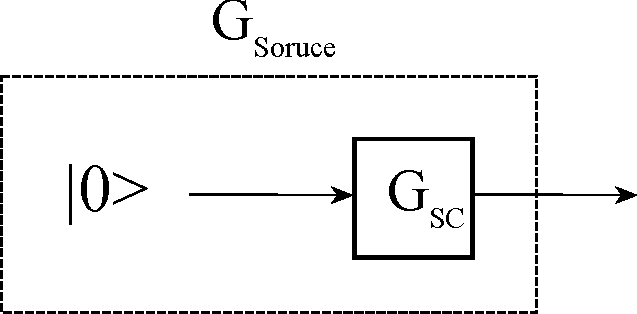
\includegraphics[width = 7.5 cm]{Soruce_term.pdf}
\caption{Non-vacuum sourced SLH model based on Fock states.
}
\label{fig:soruced_term}
\end{figure}  
SLH formalism is derived on the assumption of a vacuum input, which isn't ideal for most cases. Additional models that examine arbitrary photon input states are needed to develop SLH as seen in Figure \ref{fig:soruced_term}. One way is by proposing the source term to be coupled with a vacuum state that is fed into a sourced SLH triple for continuous-mode of coherent photons, also known as Fock states. A general case is given by  

\begin{align}
    G_{\text{Flock}} = & \ (\mathbb{1}, \lambda(t)a,0); \ \rho_{source}(t=0)= |n><n|
    \label{eq:sourced_term}
\end{align}
where a is an arbitrary system operator, $|n>$ are eigenstates of the probability density matrix, and $\lambda$ is defined as 

\begin{align*}
    \lambda(t) = \frac{\zeta(t)}{\sqrt{A(t)}} ; \ A(t) = \int_{t}^{\infty} ds |\zeta(s)|^2.
\end{align*}
For Fock states $\zeta(t)$ is the spectral density function.  
\section{EXAMPLE: Sourced Feedback of Optical Parametric Oscillator}


\begin{figure}[H]
\centering
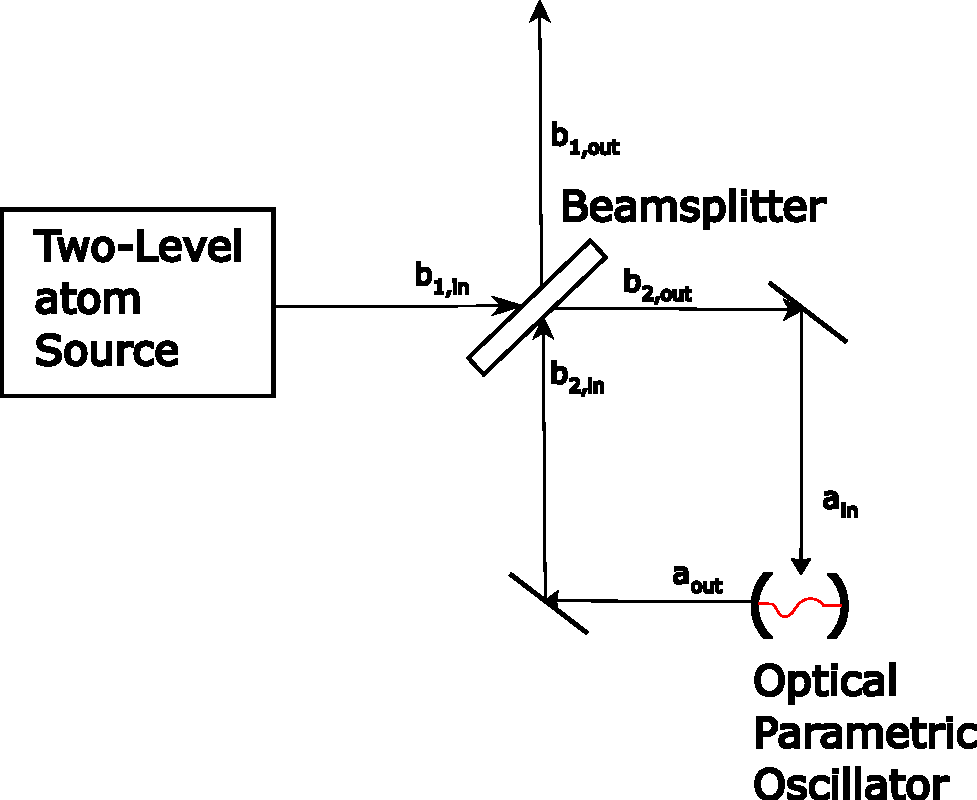
\includegraphics[width = 7.5 cm]{Example_Sourced_feedback.pdf}
\caption{Full circuit schematic of a sourced-optical parametric oscillator feedback system.
}
\label{fig:Example}
\end{figure}  

Here I have devised a simple circuit that combines the all of the basic rules (except direct coupling) and a Fock state sourced component, Figure \ref{fig:Example}. This example should highlight how to tackle the most complicated rule, the feedback reduction, alongside the concatenation and series product. The example consist of a two-level atom source with a gaussian spectral distribution ($G_{\text{Source}} $) is then pumped into the circuit component ($G_{\text{Circuit}})$ as seen in Figure \ref{fig:SLH_form}(a), which is composed of an optical parametric oscillator ($G_{text{OPO}}$) in a feedback loop with a beamsplitter ($G_B$) ($b_{2,out}$ = $a_{in}$ and $b_{2,in} = a_{out}$). Each SLH triple is defined as 

\begin{align*}
    G_{\text{Source}} = & \ ((\mathbb{1}, \lambda(t) \sigma_-,0)); \ \zeta(t)  = (\frac{\Omega^2}{2\pi})^{\frac{1}{4}}e^{\frac{-\Omega^2}{4}(t-t_c)^2} \\
    G_{\text{B}} = & \ \Bigg( \begin{pmatrix} -\sqrt{1-\eta^2} & \eta \\ \eta & \sqrt{1-\eta^2} \end{pmatrix},\begin{bmatrix} 0 \\ 0\end{bmatrix}, 0 \Bigg) \\ 
    G_{OPO} = & \ (\mathbb{1}, \sqrt{\kappa}a, i\epsilon(a^\dagger a^\dagger - a a))
\end{align*}
where $\sigma_-$ is the lowering atomic transition operator, $\Omega$ and $t_c$ are parameters for a guassian wave packet, $\eta$ is the transmission coefficient, $\kappa$ the decay rate of a photon in an optical parametric oscillator, and a is the bosonic annihilation operator for the optical parametric oscillator. The initial probability density starts at an excited state ($\rho_{source}$ = |$N_{\text{Fock}}$><e|). 
\begin{figure}[H]
\centering
   \subfloat[Broken Schematic based on Source-Circuit components.]{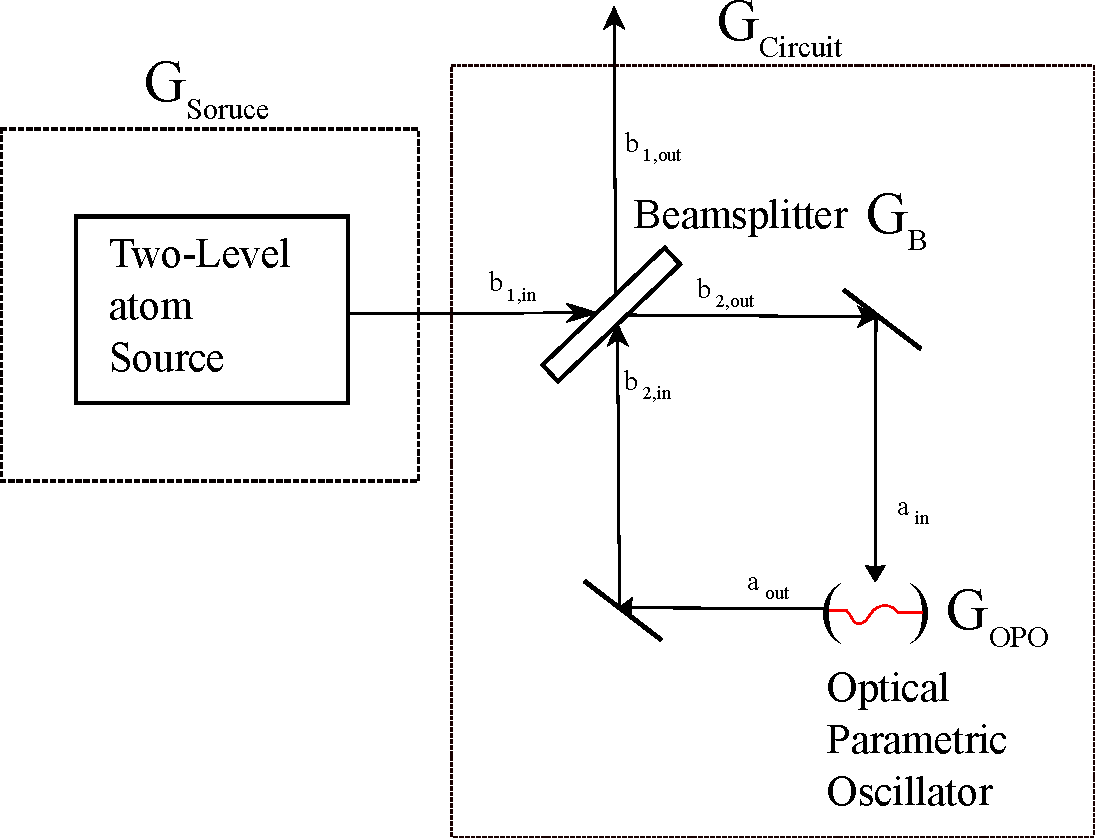
\includegraphics[width= 7.5 
   cm,keepaspectratio]{Example_Sourced_feedback2.pdf}}
     \hspace{2cm}
     \subfloat[SLH equivalent schematic.]{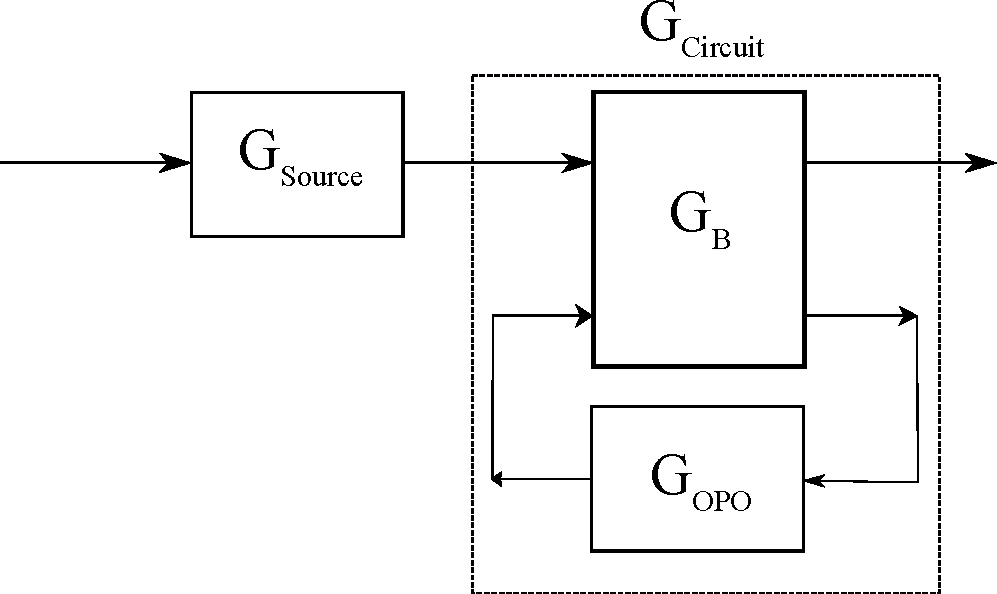
\includegraphics[width= 7.5 cm,keepaspectratio]{Example_Sourced_feedback_SLH.pdf}}

     \caption{Breakdown of a sourced-optical parametric oscillator feedback system into SLH form. The names of each component is associated with their SLH triple: Source ($G_{\text{Source}}$), beamsplitter ($G_{\text{B}}$), Optical Parametric Oscillator ($G_{\text{OPO}}$), equivalent circuit component ($G_{\text{Circuit}}$). (a) The physical system schematic. (b) The SLH equivalent of the system.}
     \label{fig:SLH_form}
\end{figure}     

NOTE: The local dimensions of the scattering matrix is the number of ports for the component. For example, the source term only has one port while the beamsplitter has two even though the identity has m by m dimensions based on the hilbert space of the sourced component. This leads to a possibility (not mentioned in any SLH paper) that we can split up a component into numerous amount of ports based on a components Hilbert space.

\section*{Sourced Component}
Following up with the sourced component (left, Figure \ref{fig:SLH_form}(b)), we then can use eq. \ref{eq:sourced_term} for a two level atom to construct an arbitrary input state. The normalization of the spectral density function A(t) is defined as 

\begin{align*}
    A(t) = & \int_{t}^{\infty} ds |(\frac{\Omega^2}{2\pi})^{\frac{1}{4}}e^{\frac{-\Omega^2}{4}(s-t_c)^2}|^2  = \frac{1}{2}(erfc(\frac{\sqrt{2}\Omega(t_c-t)}{2}+1).
\end{align*}
Thus, we can then define the time dependent dissipate term ($\lambda$(t)):

\begin{align*}
    \lambda(t) = & \ (\frac{\Omega^2}{2\pi})^{\frac{1}{4}}\frac{e^{\frac{-\Omega^2}{4}(s-t_c)^2}}{ \sqrt{\frac{1}{2}(erfc(\frac{\sqrt{2}\Omega(t_c-t)}{2}+1)}}
\end{align*}
For a two-level atom, the lower atomic transition operator is defined as
\begin{align*}
    \sigma_- =& \ \begin{pmatrix} 0 & 1 \\ 0 & 0 \end{pmatrix}
\end{align*}
The extension of a fock state input states that our initial state of $\rho_{SC}(0) = |N_{\text{Fock}}><e|$, where |e> is the excited state of the two-level atom. Based on all of this information, we can then construct the input SLH triple. 

\begin{align}
    G_{SC} = & ( \mathbb{1}, \lambda(t)\sigma_-, 0) ; \ \rho_{SC}(0) = |N_{\text{Fock}}><e|
    \label{eq:EX_source}
\end{align}
\section*{Circuit Component}
\begin{figure}[H]
\centering
   \subfloat[Reduction of circuit by $G^{1 \rightarrow 2}_{\text{unconnected}}$.]{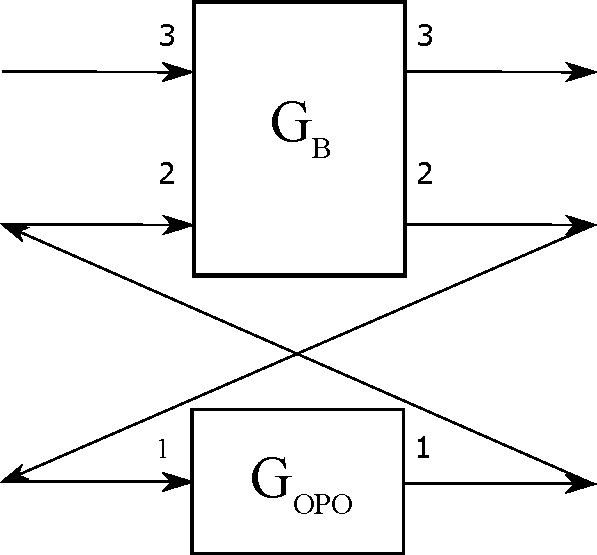
\includegraphics[width= 4 
   cm,keepaspectratio]{EX_reduction1.pdf}}
     \hspace{2cm}
     \subfloat[Reduction of circuit by $G^{1 \rightarrow 1}_{\text{B-OPO}}$.]{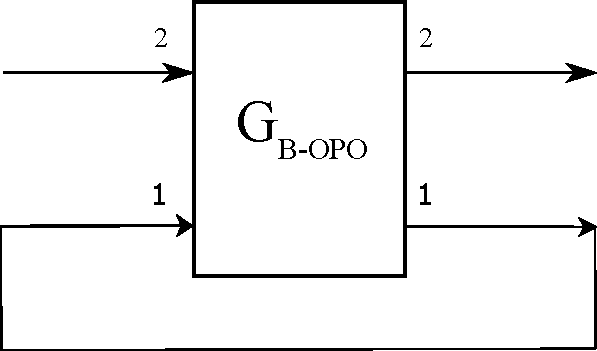
\includegraphics[width= 4 cm,keepaspectratio]{EX_reduction2.pdf}}

     \caption{Simplification of circuit component through feedbackreduction. (a) After concatenation product of unconnected beamsplitter and OPO, the output port 1 is fed into input port 2 labeled in the figure. (b) Redefining the ports as specified in Figure \ref{fig:circuit}(b), the new reduced circuit  component $G_{\text{B-OPO}}$ under goes another feedback reduction from output port 1 to input port 1.}
     \label{fig:circuit}
\end{figure}     
Now, we can simplify all of the circuit components into an equivalent SLH triple $G_{\text{Circuit}}$ which will then be in a series with the source component, Figure \ref{fig:Final_connection}. First, we need to reduced the feedback of output port 1 to input port 2 as described in Figure \ref{fig:circuit}(a) using the rules of eq. \ref{eq:feedback}. The order of reduction doesn't matter. We could have started with $2 \rightarrow 1$ instead of $1 \rightarrow 2$. I chose to reduce $1 \rightarrow 2$ first. This is done by first setting up a concatenation product of the two components as if they were unconnected.
\begin{align*}
    G_{\text{unconnected}} = & \ G_{OPO}  \boxplus G_B \\
    G_{\text{unconnected}} = & \  (\mathbb{1}, \sqrt{\kappa}a, i\epsilon(a^\dagger a^\dagger - a a))   \boxplus \Bigg( \begin{pmatrix} -\sqrt{1-\eta^2} & \eta \\ \eta & \sqrt{1-\eta^2} \end{pmatrix},\begin{bmatrix} 0 \\ 0\end{bmatrix}, 0 \Bigg)
\end{align*}
We can apply the concatenation rules from eq. \ref{eq:concatenation} to get the following result
\begin{align*}
     G_{\text{unconnected}} = & \ \Bigg( \begin{pmatrix} \mathbb{1} & 0 & 0 \\ 0 & -\sqrt{1-\eta^2} & \eta \\ 0 & \eta & \sqrt{1-\eta^2}  \end{pmatrix},\begin{bmatrix} \sqrt{\kappa}a \\ 0 \\ 0 \end{bmatrix}, H_{OPO} \Bigg).
\end{align*}
Now, we need to connect the output port 1 to input port 1 by applying eq. \ref{fig:feedback_reduction} as follows, where x = 1, y = 2, and $\mathbb{1}_{reduced} = \mathbb{1}_2$: 
\begin{align*}
    G_{\text{unconnected}}^{1 \rightarrow 2} = & \ (S_{1 \rightarrow 2}, L_{1 \rightarrow 2}, H_{1 \rightarrow 2}) =  G_{\text{B-OPO}} &  \\
    S_{1 \rightarrow 2} = & \ \begin{pmatrix}  0 & \eta \\ 0 & \sqrt{1-\eta^2}  \end{pmatrix} + \begin{bmatrix}  -\sqrt{1-\eta^2} \\ \eta \end{bmatrix} (\mathbb{1}_2-0)^{-1} \begin{bmatrix} \mathbb{1}  & 0 \end{bmatrix} & \\
    L_{1 \rightarrow 2} = & \ \begin{bmatrix}  0 \\ 0 \end{bmatrix} + \begin{bmatrix}  -\sqrt{1-\eta^2} \\ \eta \end{bmatrix} (\mathbb{1}_2-0)^{-1}(\sqrt{\kappa}a) & \\
    H_{1 \rightarrow 2} = & \ H_{OPO} + \frac{1}{2i}\Bigg( \begin{bmatrix} \sqrt{\kappa}a^\dagger  & 0 & 0 \end{bmatrix} \begin{bmatrix} 0   \\  -\sqrt{1-\eta^2} \\ \eta \end{bmatrix}  (\mathbb{1}_2)^{-1}(\sqrt{\kappa}a) \ - &  
    \\ &  (\sqrt{\kappa}a^\dagger) (\mathbb{1}_2)^{-1} \begin{bmatrix} 0  &  - \sqrt{1-\eta^2} & \eta \end{bmatrix} ) \begin{bmatrix} \sqrt{\kappa}a \\ 0 \\ 0 \end{bmatrix} \Bigg)
\end{align*}

Note:  $\mathbb{1}^{-1}_2 = \mathbb{1}_2$, and anything multiplied by the identity is itself. Notice that the reduced hamiltonian is just $H_{OPO}$. Thus, the result of the first feedback reduction as shown in Figure \ref{fig:circuit}(b) is given by 
\begin{align}
    G_{\text{B-OPO}} = & \ \Bigg( \begin{pmatrix} -\sqrt{1-\eta^2} & \eta \\ \eta & \sqrt{1-\eta^2} \end{pmatrix}, \begin{bmatrix}  -\sqrt{1-\eta^2}(\sqrt{\kappa}a) \\ \eta(\sqrt{\kappa}a) \end{bmatrix}, H_{OPO}  \Bigg)
    \label{eq:EX_reduced_1}
\end{align}
Finally, we can do one more feedback reduction to obtain the equivalent circuit SLH triple. Redefining the port as described in Figure \ref{fig:circuit}(b), we'll do a feedback reduction of $1 \rightarrow 1$ using eq. \ref{eq:feedback} with x = 1 and y = 1, and the new reduced identity $\mathbb{1}_{reduced} = 1$. We'll use the result obtained in eq. \ref{eq:EX_reduced_1} as shown in Figure \ref{fig:circuit}(b).
\begin{align*}
    G_{\text{B-OPO}}^{1 \rightarrow 1} = & \ (S_{1 \rightarrow 1}, L_{1 \rightarrow 1}, H_{1 \rightarrow 1}) =  G_{\text{Circuit}} & \\
    S_{1 \rightarrow 1} = & \ \sqrt{1-\eta^2} + \eta (1+\sqrt{1-\eta^2})^{-1}(\eta)& \\
    L_{1 \rightarrow 1} = & \ \eta(\sqrt{\kappa}a) + \eta (1+\sqrt{1-\eta^2})^{-1}(-\sqrt{1-\eta^2}(\sqrt{\kappa}a)) & \\
    H_{1 \rightarrow 1} = & \ H_{OPO} + \frac{1}{2i}\Bigg( \begin{bmatrix} -\sqrt{1-\eta^2}\sqrt{\kappa}a^\dagger  & \eta \sqrt{\kappa}a^\dagger \end{bmatrix} \begin{bmatrix}   -\sqrt{1-\eta^2} \\ \eta \end{bmatrix}  (1+\sqrt{1-\eta^2})^{-1} ( -\sqrt{1-\eta^2}\sqrt{\kappa}a) \ - &  
    \\ &  ( -\sqrt{1-\eta^2}\sqrt{\kappa}a^\dagger) (1+\sqrt{1-\eta^2})^{-1} \begin{bmatrix}  - \sqrt{1-\eta^2} & \eta \end{bmatrix} ) \begin{bmatrix} -\sqrt{1-\eta^2}(\sqrt{\kappa}a) \\ \eta(\sqrt{\kappa}a) \end{bmatrix} \Bigg)& 
\end{align*}
After basic algebraic operations we'll arrive at the equivalent circuit SLH triple. 
\begin{align}
    G_{\text{Circuit}} = & \ \Bigg( \mathbb{1}, \ell \sqrt{\kappa}a ,H_{OPO}\Bigg); \ \ell = \frac{\eta}{(1+\sqrt{1-\eta^2})}
    \label{eq:Ex_Circuit}
\end{align}
\section*{Total SLH Triple}

\begin{figure}[H]
\centering
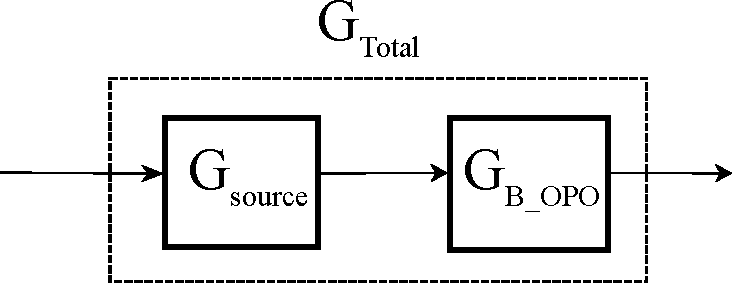
\includegraphics[width = 9 cm]{Example_Sourced_feedback_final.pdf}
\caption{Series product of the source term with the reduced $G_{\text{B-OPO}}$.
}
\label{fig:Final_connection}
\end{figure}  

We have broken down every component into two basic SLH triples: $G_{\text{Source}}$ and $G_{\text{Circuit}}$. Based on Figure \ref{fig:Final_connection}, we can use eq. \ref{eq:series} to get the total system SLH triple with eq. \ref{eq:EX_source} and \ref{eq:Ex_Circuit}. The final result is given by 
\begin{align*}
    G_{\text{Total}} = & \ G_{\text{Circuit}} \triangleleft G_{\text{SC}} \\
    G_{\text{Total}} = & \ \Bigg( \mathbb{1}, \ell \sqrt{\kappa}a ,H_{OPO}\Bigg) \triangleleft \Bigg( \mathbb{1}, \lambda(t)\sigma_-, 0 \Bigg) \\ 
    G_{\text{Total}} = & \ \Bigg( \mathbb{1}\mathbb{1}, \ell \sqrt{\kappa}a +  \mathbb{1} \lambda(t)\sigma_-,H_{OPO} + \frac{1}{2i}(\ell \sqrt{\kappa}a^\dagger \mathbb{1}  \lambda(t)\sigma_- - \lambda^*(t)\sigma_-^\dagger \mathbb{1}  \ell \sqrt{\kappa}a) \Bigg)
\end{align*}
\begin{align}
    G_{\text{Total}} = & \ \Bigg( \mathbb{1}, \ell \sqrt{\kappa}a + \lambda(t)\sigma_-, i\epsilon(a^\dagger a^\dagger - a a) + \frac{\ell \sqrt{\kappa}}{2i}(a^\dagger \lambda(t)\sigma_- - \lambda^*(t)\sigma_-^\dagger a) \Bigg)
    \label{eq:EX_FINAL_RESULT}
\end{align}

I hope this example is able to capture the core aspects of SLH formalism. As seen in this example, we can tackle difficult quantum based circuits using rudimentary, algebraic operations. In later examples, hopefully I'll be able to show you how to derive each SLH operation and explain more in detail. Alongside with this document, I'll have the jupyter notebook example that numerically solves the master equation using QuTip with this SLH triple. All rules were derived from Joshua Combes SLH tutorial ("The SLH framework for modeling quantum input-output networks"). 




\bibliography{Work}
\end{document}
